%! Addition and Multiplication Rules — Unit 3, Lesson 3.3 — Guided Notes & Practice
% THE in-class document, in the MAIN IDEAS / NOTES shape (LESSON_SHAPE.md §1): the vocabulary
% box, the hook, then ONE two-column guidednotes table. Problems run 1..15. Unit 3 timing
% (5/45/5/5): I do ~25 min (rows 1-4, problems 1-11), Guided Practice ~20 (problems 12-15).
% 4 pages at 12pt — a ceiling (10-page packet, LESSON_SHAPE.md §1).
%   I DO   : the teacher reads the definition, marks up the display, works 1, 3, 5, 7, 9.
%   WE DO  : the class works the rest of each grid; Guided Practice (12-15) worked together.
%   YOU DO : nothing on this page — ../homework/ IS the individual practice.
% THE TRAPS: problem 2 (adding without subtracting gives 1.1) and problem 6 (adding the two
% draws for "at least one": 6/10).
% THE CRUX: problem 10 (row 4): N and T cannot happen together, the hook vote re-taken, and
% P(N and T) = 0 against P(N)P(T) = 0.05 shows they are DEPENDENT. Problem 15 transfers it.
%
% THE DATA (all verified in Python)
%   Drum, 40 tickets: S student 24, E early 20, both 12, S only 12, E only 8, neither 8.
%     P(S)=.6, P(E)=.5, P(both)=.3 = P(S)P(E) -> independent; P(S or E)=.8; 1-.2=.8.
%     N ninth grader 8 (.2), T twelfth grader 10 (.25), both 0, neither 22 (.55); N or T .45;
%     P(N)P(T)=.05. A adult 16 (.4), complement of S; P(S)P(A)=.24.
%   Bowl, 10 tickets: 3 gold, 7 white, two draws.
%     put back: GG 9/100; at least one gold 1-49/100=51/100 (= 3/10+3/10-9/100).
%     kept out: second-stage 2/9, 7/9, 3/9, 6/9; GG 6/90 = 1/15, about 0.067.
%   Commute: P(R)=.4, P(L)=.2, both .15; R only .25, L only .05, neither .55.
%     R or L .45; P(R)P(L)=.08 -> dependent; two days LL .04, at least one 1-.64=.36;
%     P(Y)=.1 (bus early), P(L and Y)=0, P(L)P(Y)=.02 -> dependent.
%
% PAGE LOCKSTEP with notes_key/ (generated by templates/lesson/mkkey.py). KEEP EVERY \pcell ON
% ONE SOURCE LINE. Inside a cell `\\` ENDS THE ROW; a row cannot break across pages.
\documentclass[12pt]{article}
\usepackage{saar-article}
\usepackage{saar-boxes}
\newcommand{\TallMath}[1]{$\displaystyle #1\rule[-1.4em]{0pt}{3.2em}$}
% Vocabulary rows: FIXED-HEIGHT, term label and open writing space, no rule line. Copied from
% unit01/lesson02/notes/main.tex. Keep key definitions to two lines.
\newcommand{\termrowheight}{2.3cm}
\newlength{\termrowinset}\setlength{\termrowinset}{7pt}
\newcommand{\vterm}[1]{%
  \par\noindent\begin{minipage}[t][\termrowheight][t]{\linewidth}%
    \vspace*{\termrowinset}%
    \textbf{\textcolor{cerulean}{#1:}}%
  \end{minipage}\par}
\newcommand{\vtermans}[2]{%
  \par\noindent\begin{minipage}[t][\termrowheight][t]{\linewidth}%
    \vspace*{\termrowinset}%
    \textbf{\textcolor{cerulean}{#1:}}\quad\ans{#2}%
  \end{minipage}\par}

\begin{document}

\pageheader{Unit 3, Lesson 3.3}{Guided Notes \& Practice}
% NAMESTRIP: no \namedateperiod here. The student writes their name once, on the
% cover this component is stapled behind.

\vspace{0.15in}

\boxguard[16]
\begin{vocabbox}
\small
Fill in each term \textbf{as we name it} in the notes below.
\vterm{Addition rule}
\vterm{Independent events}
\vterm{Dependent events}
\vterm{Multiplication rule}
\end{vocabbox}

\boxguard[12]
\begin{hookbox}
\small
The concert raffle draws one winning ticket. Event $N$: the ticket was sold to a ninth grader.
Event $T$: it was sold to a twelfth grader. One ticket cannot be both. Devon says,
\emph{``They can't happen together, so they have nothing to do with each other. They must be
independent.''}

\vspace{3pt}
\textbf{Is Devon right?} Circle one: \quad independent \qquad dependent \qquad can't tell
\quad --- and say why. We vote again at problem~10.
\par\writelines{2}
\end{hookbox}

\small
\begin{guidednotes}
% ── ROW 1: general addition rule on a pre-drawn Venn ─────────────────────────
\mainidea[Subtract the overlap]{Addition Rule} &
The raffle drum holds $40$ tickets, and one is drawn at random. ``$A$ or $B$'' means at least
one of the two happens. The \textbf{addition rule} is
$P(A \text{ or } B) = P(A) + P(B) - P(A \text{ and } B)$: the overlap is subtracted because
those outcomes sit inside both circles.
\\
& {\centering
\begin{tikzpicture}[x=1cm, y=1cm]
  \draw[thick, charcoal] (0,0) rectangle (11.6,3.3);
  \fill[cerulean, fill opacity=0.18] (5.0,1.55) circle[radius=1.4];
  \fill[goldacc, fill opacity=0.25] (7.0,1.55) circle[radius=1.4];
  \draw[thick, cerulean] (5.0,1.55) circle[radius=1.4];
  \draw[thick, goldacc] (7.0,1.55) circle[radius=1.4];
  \node[font=\footnotesize\bfseries, anchor=east] at (3.9,3.0) {$S$: sold to a student};
  \node[font=\footnotesize\bfseries, anchor=west] at (8.1,3.0) {$E$: sold early};
  \node[font=\Large\bfseries] at (4.3,1.55) {12};
  \node[font=\Large\bfseries] at (6.0,1.55) {12};
  \node[font=\Large\bfseries] at (7.7,1.55) {8};
  \node[font=\Large\bfseries] at (10.5,0.75) {8};
  \node[font=\scriptsize\itshape] at (10.5,0.3) {neither};
  \node[font=\footnotesize, anchor=south west] at (0.08,0.05) {$40$ tickets in all};
  \node[font=\footnotesize, align=center, text width=3.1cm] at (1.75,1.6) {Adding the circles counts each overlap ticket \labelbox{0.9cm}{}\ times};
\end{tikzpicture}\par}
\\
& \notesprompt{Give each probability as a decimal, in context.}
\begin{probgrid}{|Y|Y|}
\pcell{1}{Find $P(S \text{ or } E)$ with the addition rule. Check it by counting tickets.}{2.1cm}{} & \pcell{2}{Jamal adds $P(S) + P(E)$ and gets $1.1$. How do you know he is wrong, and what did he forget?}{2.1cm}{} \\ \hline
\end{probgrid}
\\ \hline
% ── ROW 2: mutually exclusive, overlap 0; complement rule for "at least one" ─
\mainidea[Overlap of zero]{Mutually Exclusive} &
Two events are \textbf{mutually exclusive} when they cannot happen together, so
$P(A \text{ and } B) = 0$ and the addition rule shortens to $P(A \text{ or } B) = P(A) + P(B)$.
The complement rule finds ``at least one'' from its opposite:
$P(\text{at least one}) = 1 - P(\text{none})$.
\\
& {\centering
\begin{tikzpicture}[x=1cm, y=1cm]
  \draw[thick, charcoal] (0,0) rectangle (11.6,2.95);
  \fill[cerulean, fill opacity=0.18] (2.9,1.2) circle[radius=1.1];
  \fill[goldacc, fill opacity=0.25] (7.7,1.2) circle[radius=1.1];
  \draw[thick, cerulean] (2.9,1.2) circle[radius=1.1];
  \draw[thick, goldacc] (7.7,1.2) circle[radius=1.1];
  \node[font=\footnotesize\bfseries] at (2.9,2.65) {$N$: sold to a ninth grader};
  \node[font=\footnotesize\bfseries] at (8.1,2.65) {$T$: sold to a twelfth grader};
  \node[font=\Large\bfseries] at (2.9,1.2) {8};
  \node[font=\Large\bfseries] at (7.7,1.2) {10};
  \node[font=\Large\bfseries] at (10.5,0.7) {22};
  \node[font=\scriptsize\itshape] at (10.5,0.27) {neither};
  \node[font=\footnotesize, anchor=south west] at (0.08,0.05) {$40$ tickets};
\end{tikzpicture}\par}
\\
& \begin{probgrid}{|Y|Y|}
\pcell{3}{Find $P(N \text{ or } T)$. Why is nothing subtracted this time?}{2.1cm}{} & \pcell{4}{Back to row 1's Venn. Use the complement rule to find the probability the ticket is $S$, $E$, or both.}{2.1cm}{} \\ \hline
\end{probgrid}
\\ \hline
% ── ROW 3: multiplication rule on a pre-drawn tree ───────────────────────────
\mainidea[Multiply along the branches]{Trees} &
Two events are \textbf{independent} when one happening does not change the probability of the
other, and \textbf{dependent} when it does. The \textbf{multiplication rule} gives the chance
both happen: for independent events, $P(A \text{ and } B) = P(A) \cdot P(B)$; for dependent
events, the second factor is $B$'s probability \emph{after} $A$ happened. The final-round bowl
holds $10$ tickets, $3$ gold and $7$ white, and two tickets are drawn, one after the other.
\\
& {\centering
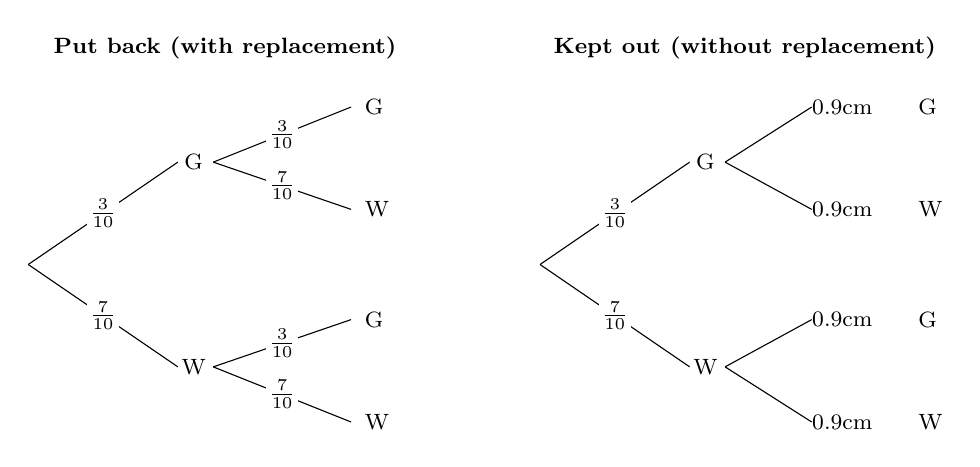
\begin{tikzpicture}[x=1cm, y=1cm, every node/.style={font=\footnotesize}]
  \tikzset{br/.style={fill=white, inner sep=1pt}}
  % put back
  \node[font=\footnotesize\bfseries] at (2.5,2.75) {Put back (with replacement)};
  \draw (0,0) -- node[br]{$\frac{3}{10}$} (1.9,1.3);
  \draw (0,0) -- node[br]{$\frac{7}{10}$} (1.9,-1.3);
  \node at (2.1,1.3) {G};  \node at (2.1,-1.3) {W};
  \draw (2.35,1.3) -- node[br]{$\frac{3}{10}$} (4.1,2.0);
  \draw (2.35,1.3) -- node[br]{$\frac{7}{10}$} (4.1,0.7);
  \draw (2.35,-1.3) -- node[br]{$\frac{3}{10}$} (4.1,-0.7);
  \draw (2.35,-1.3) -- node[br]{$\frac{7}{10}$} (4.1,-2.0);
  \node[anchor=west] at (4.15,2.0) {G};   \node[anchor=west] at (4.15,0.7) {W};
  \node[anchor=west] at (4.15,-0.7) {G};  \node[anchor=west] at (4.15,-2.0) {W};
  % kept out
  \begin{scope}[xshift=6.5cm]
  \node[font=\footnotesize\bfseries] at (2.6,2.75) {Kept out (without replacement)};
  \draw (0,0) -- node[br]{$\frac{3}{10}$} (1.9,1.3);
  \draw (0,0) -- node[br]{$\frac{7}{10}$} (1.9,-1.3);
  \node at (2.1,1.3) {G};  \node at (2.1,-1.3) {W};
  \draw (2.35,1.3) -- (3.45,2.0);  \draw (2.35,1.3) -- (3.45,0.7);
  \draw (2.35,-1.3) -- (3.45,-0.7);  \draw (2.35,-1.3) -- (3.45,-2.0);
  \node[inner sep=0pt, anchor=west] at (3.45,2.0) {\labelbox{0.9cm}{}};
  \node[inner sep=0pt, anchor=west] at (3.45,0.7) {\labelbox{0.9cm}{}};
  \node[inner sep=0pt, anchor=west] at (3.45,-0.7) {\labelbox{0.9cm}{}};
  \node[inner sep=0pt, anchor=west] at (3.45,-2.0) {\labelbox{0.9cm}{}};
  \node[anchor=west] at (4.68,2.0) {G};   \node[anchor=west] at (4.68,0.7) {W};
  \node[anchor=west] at (4.68,-0.7) {G};  \node[anchor=west] at (4.68,-2.0) {W};
  \end{scope}
\end{tikzpicture}\par}
\\
& \notesprompt{Multiply along the path. Fractions are fine.}
\begin{probgrid}{|Y|Y|}
\pcell{5}{Ticket put back. Find $P(\text{gold, then gold})$.}{2.0cm}{} & \pcell{6}{Ticket put back. Ana says $P(\text{at least one gold}) = \frac{3}{10} + \frac{3}{10} = \frac{6}{10}$. Find the right value. What did she count twice?}{2.4cm}{} \\ \hline
\end{probgrid}
\\
& \begin{probgrid}*{|Y|Y|}
\pcell{7}{Ticket kept out. Fill in the four boxes on the tree, then find $P(\text{gold, then gold})$.}{2.0cm}{} & \pcell{8}{Compare the chance of a second gold after a first gold on each tree. Which tree's draws are independent? Which are dependent?}{2.0cm}{} \\ \hline
\end{probgrid}
\\ \hline
% ── ROW 4: classify by computation — THE CRUX ────────────────────────────────
\mainidea[Compute, then name]{Four Words} &
Classify a pair of events by \textbf{computing}, not by how the words sound.
\par\vspace{4pt}
\fcolorbox{cerulean}{frost}{\parbox{\dimexpr\linewidth-2\fboxsep-2\fboxrule\relax}{\renewcommand{\arraystretch}{1.2}%
\begin{tabular}{@{} l l @{}}
\textbf{Mutually exclusive} & $P(A \text{ and } B) = 0$ \\
\textbf{Complementary} & mutually exclusive and $P(A) + P(B) = 1$ \\
\textbf{Independent} & $P(A \text{ and } B) = P(A) \cdot P(B)$ \\
\textbf{Dependent} & $P(A \text{ and } B) \neq P(A) \cdot P(B)$ \\
\end{tabular}}}
\\
& {\centering
\begin{tikzpicture}[scale=0.9]
  \draw[thick, charcoal] (0,0) rectangle (6.4,2.9);
  \fill[cerulean, fill opacity=0.18] (2.4,1.35) circle[radius=1.15];
  \fill[goldacc, fill opacity=0.25] (4.0,1.35) circle[radius=1.15];
  \draw[thick, cerulean] (2.4,1.35) circle[radius=1.15];
  \draw[thick, goldacc] (4.0,1.35) circle[radius=1.15];
  \node[font=\footnotesize\bfseries] at (0.35,2.6) {$S$};
  \node[font=\footnotesize\bfseries] at (6.05,2.6) {$E$};
  \node[font=\normalsize\bfseries] at (1.85,1.35) {.30};
  \node[font=\normalsize\bfseries] at (3.2,1.35) {.30};
  \node[font=\normalsize\bfseries] at (4.55,1.35) {.20};
  \node[font=\normalsize\bfseries] at (5.85,0.35) {.20};
  \begin{scope}[xshift=7.0cm]
  \draw[thick, charcoal] (0,0) rectangle (6.4,2.9);
  \fill[cerulean, fill opacity=0.18] (1.6,1.35) circle[radius=1.0];
  \fill[goldacc, fill opacity=0.25] (4.2,1.35) circle[radius=1.0];
  \draw[thick, cerulean] (1.6,1.35) circle[radius=1.0];
  \draw[thick, goldacc] (4.2,1.35) circle[radius=1.0];
  \node[font=\footnotesize\bfseries] at (0.35,2.6) {$N$};
  \node[font=\footnotesize\bfseries] at (3.0,2.6) {$T$};
  \node[font=\normalsize\bfseries] at (1.6,1.35) {.20};
  \node[font=\normalsize\bfseries] at (4.2,1.35) {.25};
  \node[font=\normalsize\bfseries] at (5.85,0.35) {.55};
  \end{scope}
\end{tikzpicture}\par}
\\
& \begin{probgrid}{|Y|Y|}
\pcell{9}{$S$ and $E$. Compute $P(S \text{ and } E)$ and $P(S) \cdot P(E)$. Which words fit?}{2.6cm}{} & \pcell{10}{\textbf{Vote again on Devon.} Compute $P(N \text{ and } T)$ and $P(N) \cdot P(T)$. If $N$ happened, what is the chance of $T$ now?}{2.6cm}{} \\ \hline
\end{probgrid}
\\
& \fcolorbox{cerulean}{frost}{\parbox{\dimexpr\linewidth-2\fboxsep-2\fboxrule\relax}{\centering
\textbf{Mutually exclusive is not independent. When two events that each have some chance
cannot happen together, knowing one happened tells you the other did not: they are dependent.}}}
\\
& \begin{probgrid}{|Y|}
\pcell{11}{Every ticket was sold to a student ($S$) or an adult ($A$, $16$ of the $40$), never both. Compute $P(S) + P(A)$, $P(S \text{ and } A)$, and $P(S) \cdot P(A)$. Which words fit?}{2.0cm}{} \\ \hline
\end{probgrid}
\\ \hline
% ── ROW 5: GUIDED PRACTICE — we do, together, a fresh context ────────────────
\mainidea[Guided practice]{Rain and the Bus} &
Leah rides the bus to school. On a school morning, $R$ is the event that it rains and $L$ is the
event that her bus is late. We work these together.
\\
& {\centering
\begin{tikzpicture}[x=1cm, y=1cm]
  \draw[thick, charcoal] (0,0) rectangle (11.6,2.8);
  \fill[cerulean, fill opacity=0.18] (4.9,1.4) circle[radius=1.2];
  \fill[goldacc, fill opacity=0.25] (6.7,1.4) circle[radius=1.2];
  \draw[thick, cerulean] (4.9,1.4) circle[radius=1.2];
  \draw[thick, goldacc] (6.7,1.4) circle[radius=1.2];
  \node[font=\footnotesize\bfseries, anchor=east] at (3.75,2.4) {$R$: it rains};
  \node[font=\footnotesize\bfseries, anchor=west] at (7.85,2.4) {$L$: the bus is late};
  \node[font=\Large\bfseries] at (4.3,1.4) {.25};
  \node[font=\Large\bfseries] at (5.8,1.4) {.15};
  \node[font=\Large\bfseries] at (7.3,1.4) {.05};
  \node[font=\Large\bfseries] at (10.5,0.7) {.55};
  \node[font=\scriptsize\itshape] at (10.5,0.27) {neither};
\end{tikzpicture}\par}
\\
& \begin{probgrid}{|Y|Y|}
\pcell{12}{Find $P(R \text{ or } L)$ with the addition rule. Then say what it means for Leah's mornings.}{2.2cm}{} & \pcell{13}{Compute $P(R \text{ and } L)$ and $P(R) \cdot P(L)$. Are rain and a late bus independent or dependent? What does that mean here?}{2.2cm}{} \\ \hline
\end{probgrid}
\\
& \begin{probgrid}*{|Y|Y|}
\pcell{14}{Mornings are independent. Over two mornings, find $P(\text{late both})$ and $P(\text{late at least once})$.}{2.2cm}{} & \pcell{15}{$P(\text{early}) = .1$ ($Y$). A bus can't be both, so Theo says $L$ and $Y$ are independent. Compute; answer him.}{2.2cm}{} \\ \hline
\end{probgrid}
\\ \hline
\end{guidednotes}

% ── THE NOTES END AT GUIDED PRACTICE ─────────────────────────────────────────
% There is deliberately no "you do" here: ../homework/ is the individual practice,
% assigned at Close & Assign and done outside class.

\end{document}
